\chapter{Lecture 14 - Combined Cycles}
\label{ch:ch14}
\section{Objectives}
The objectives of this lecture are:
\begin{enumerate}
\item Describe an example combined cycle and illustrate key analysis methods
\item Illustrate incorporation of hydraulic pressure drops in a Brayton cycle.
\end{enumerate}

\index{Combined cycle}
\section{Combined Cycle by Example}
\newthought{A different approach to} improving the thermal efficiency of the nuclear energy conversion process is to use a \emph{combined cycle}.  In this concept, we use thermal energy remaining in the working fluid after expansion in a turbine as input into \emph{another} thermodynamic cycle; a portion of that heat is thus converted to work.  Since this was done with no additional heat being added, thermal efficiency is improved by increasing the net specific work.  Compare this with regenerating Brayton cycles that increase thermal efficiency by reducing the amount of heat that must be added per unit mass of working fluid with no change in specific work output.  In principle there are many different types of combined cycles one might explore but in this course we will focus on Brayton-Rankine combined cycles where waste heat from a Brayton cycle is used as heat input for a Rankine ``bottoming cycle.''  One such cycle\cite{forsberg2014meeting} is illustrated in the schematic in Figure \ref{fig:FHR_schematic}.  Key system parameters are summarized in Table \ref{tab:FHR_params}.  State point property data are tabulated in Figure \ref{fig:combined_cycle_SPT}.

\newthought{One notable feature} of this analysis is the inclusion of hydraulic pressure losses.  In previous cycle analyses, it was assumed either explicitly or implicitly that heat transfer processes in a Brayton cycle would take place at constant pressure.  In reality, viscous flow through complex heat exchanger geometry results in frictional pressure drops.  



\begin{figure}
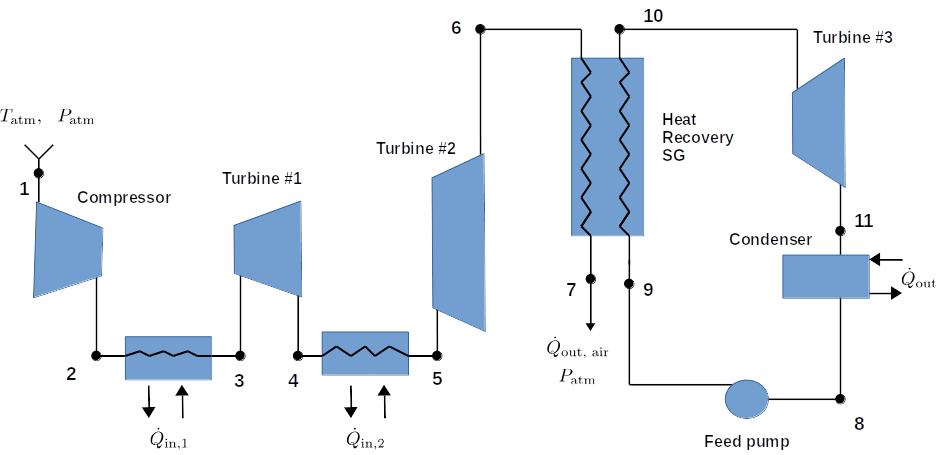
\includegraphics{FHR_schematic.png}
\caption{Schematic of a FHR combined cycle}
\label{fig:FHR_schematic}
\end{figure}

\begin{margintable}
\begin{tabular}{lc}
\toprule
Property & Value \\
\midrule
$T_{\text{atm}}$ & 15$^{\circ}C$ \\
$P_{\text{atm}}$ & 101.3 kPa \\
$T_{\text{max}}$ & 770$^{\circ}C$ \\
$T_{\text{exh,air}}$ & 250$^{\circ}C$ \\
$r_{p}$ & 17 \\
$r_{e1}$ & 4 \\
$\eta_T$ & 0.92 \\
$\eta_c$ & 0.89 \\
$eta_p$ & 0.80 \\
\bottomrule
\end{tabular}
\caption{FHR Parameters}
\label{tab:FHR_params}
\end{margintable}

\begin{figure}
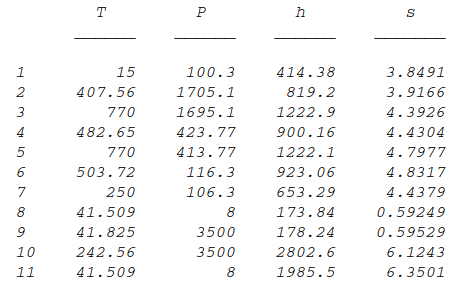
\includegraphics{combined_cycle_SPT.png}
\caption[][5cm]{State point property data for FHR.}
\label{fig:combined_cycle_SPT}
\end{figure}

Take for example air flow into the compressor.  Air is drawn from the atmosphere, here assumed to be at standard temperature and pressure, through inlet ducting which, besides directing air flow to the compressor inlet would perform other essential functions such as preventing the introduction of harmful foreign objects into the machine. It should be clear that the fluid arriving at state point 1 will have lost some energy in the process of traversing the dampers, filters, and various duct work. That energy loss will be manifest as a reduction in static pressure.  As is evident from the state point table, the pressure at state point 1 is listed as 100.3 kPa---1 kPa lower than atmospheric pressure.  

Similarly, air flowing from the compressor discharge through the heat exchanger between state points 2 and 3 cannot be expected to pass through the complex heat exchanger geometry without some flow-energy losses.  For this problem, the pressure loss $\Delta P_{HX} = P_3 - P_2 = 10$kPa.  In upcoming lectures we will examine techniques for quantifying hydraulic pressure losses in the context of diabatic flows such as this one.

For the purposes of lectures and associated homework problems, we will take hydraulic pressure losses to be given parameters.  The losses will be expressed either as:
\begin{enumerate}
\item fixed given $\Delta P$ as with the two cases just described; or
\item a fractional pressure drop where the $\Delta P$ for a given process will be given as a fraction of the state point pressure at the process inlet. 
\end{enumerate}
With this methodology it is often possible and preferable to compute all state point pressures first before determining all other state point properties.

\newthought{The hydraulic pressure drops} have a significant effect on net specific work and thermal efficiency.  If, as we have done up until now, we assumed no hydraulic pressure losses throughout the system, the net specific work and thermal efficiency would be 324.4 kJ/kg and 44.7\%.  Including pressure losses, net specific work is 300.5 kJ/kg and thermal efficiency is only 41.4\%.

\subsection{Analysis of Combined Cycle}
There are a few details to the analysis of a combined cycle that are best communicated simply by doing the calculations.  

\begin{enumerate}
\item What is the ratio of the air and steam mass flow rates?

This is determined through an energy balance for the heat recovery steam generator expressed in Equation \ref{eq:ebal_hrsg}

\begin{equation}
\dot{m}_a (h_6 - h_7) = \dot{m}_s (h_{10}-h_9)
\label{eq:ebal_hrsg}
\end{equation}
For this problem, therefore:
$$ \frac{\dot{m}_s}{\dot{m}_a} = \frac{h_6 - h_7}{h_{10}-h_9}$$

\item What is the net specific work for this cycle?

In this case, we need to be a bit more specific about what we mean by ``specific work.'' Normally the specific work is the power divided by the mass flow rate of the working fluid; but in this cycle we have two different working fluids with generally different flow rates.  In order to perform a consistent analysis of the cycle we should define specific work to be power per unit mass flow rate of \emph{one} of the working fluids; for this cycle we will choose the air in the Brayton cycle as the reference working fluid.

\begin{align*}
w_{\text{net}} &= \frac{\dot{W}}{\dot{m}_a} \\
               &= w_c + w_{T_1} + w_{T_2} + w_{T_3} + w_p \\
&=(h_1 - h_2) + (h_3 - h_4) + (h_5 - h_6) + \frac{\dot{m}_s}{\dot{m}_a}(h_{10}-h_{11}) + \frac{\dot{m}_s}{\dot{m}_a}(h_8 - h_9)\\ 
\end{align*}

\item What is the net specific heat added?

For this cycle, heat is added only in the processes from state points 2 to 3 and 4 to 5.\sidenote{\textbf{Question:} Why do you not count the heat exchanged in the heat recovery SG?}  Since air is the only working fluid involved in these processes, this calculation is carried out as before:

$$q_s = (h_3 - h_2) + (h_5 - h_4)$$

\item What is the cycle thermal efficiency?

Since we have taken care to consistently calculate both the net specific heat added and the net specific work in terms of the mass flow rate of air, we can compute thermal efficiency in the usual way:

$$\eta_{\text{TH}} = \frac{w_{\text{net}}}{q_s}$$

\item What would the thermal efficiency be without the Rankine ``Bottoming'' cycle?

For this calculation we would simply eliminate the specific work of the Rankine cycle turbine and pump from the net work calculation.

\end{enumerate}
